\section{Petalinux Tool Flow}
\label{sec:Petalinux_Toolflow}
PetaLinux ist ein Embedded Linux Software Development Kit (SDK), das auf FPGA-basierte System-on-a-Chip (SoC)-Designs abzielt. Petalinux (2020). Es erstellt das Root-Dateisystem unter Verwendung von Yocto, es setzt praktisch auf Yocto auf. Unter PetaLinux versteht man eine Reihe von High-Level-Befehlen, die auf der Yocto-Linux-Distribution aufbauen. Die PetaLinux-Werkzeuge können zur Anpassung, Erstellung und Bereitstellung von Embedded Linux-Lösungen/Linux-Images für Xilinx-Prozessorsysteme verwendet werden. So arbeitet PetaLinux mit den Hardware-Design-Tools von Xilinx (z.B. Vivado) zusammen, um die Entwicklung von Linux-Systemen für unseren Zynq UltraScale+MPSoC zu erleichtern.\\
Ein wesentlicher Vorteil von petalinux ist, dass es eine Reihe von vereinfachten Befehlen enthält, die für das Booten und die Integration von HW- und SW-Projekten sehr nützlich sind. In Abbildung ~\ref{fig:petalinux:tool:flow} sehen Sie einen Überblick über den PetaLinux-Werkzeugfluss auf oberster Ebene.
	
\begin{figure}[h]
	\begin{center}
		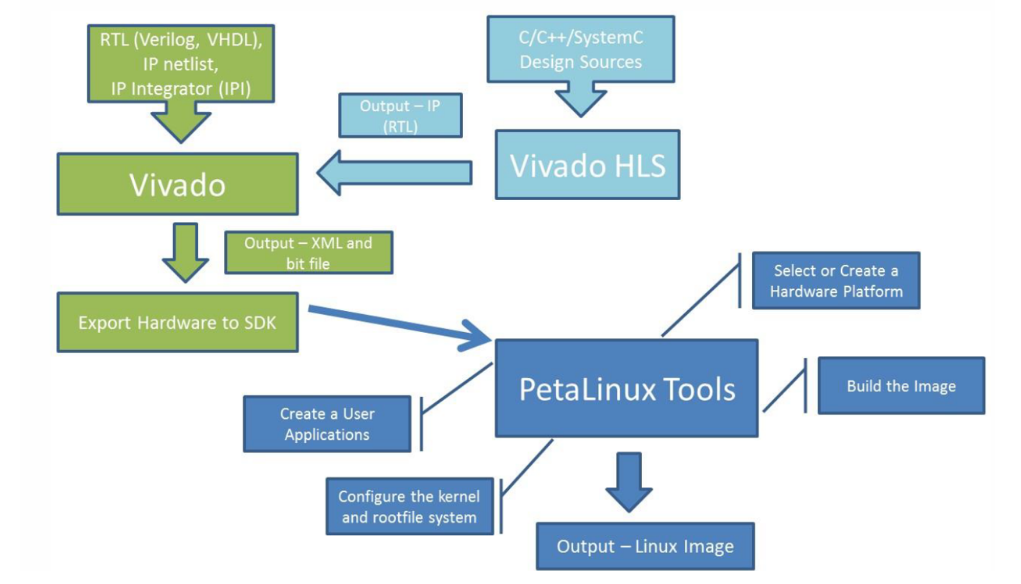
\includegraphics[width=1.1\textwidth]{./images/petalinux-toolflow.jpg}
	\end{center}
	\vspace{-5pt}
	\caption[PetaLinux-Werkzeugfluss]{Überblick über den PetaLinux-Werkzeugfluss [\cite{petailinuxtool}]} % Eckige Klammer (optional): Caption-Text in Abbildungsverzeichnis
	\label{fig:petalinux:tool:flow}
	\vspace{-5pt}
\end{figure}

Wie man in der Abbildung ~\ref{fig:petalinux:tool:flow} sehen kann, ist es möglich, mit Vivado erstellte Hardware-Designs in petalinux zu importieren, einige Anwendungen in petalinux einzubinden und ein Linux-Image zu erstellen.  

\subsubsection{Petalinux Installation}
Wie jedes Build-System benötigt petalinux viele Ressourcen auf Ihrem PC. Um die Kompilierzeit deutlich zu reduzieren, ist es daher sinnvoll, einen Computer mit folgenden Eigenschaften zu verwenden.\cite{Xilinx2020}

\begin{itemize}
	\item 8 GB RAM
	\item 2 GHz CPU-Takt oder gleichwertig
	\item 100 GB freier HDD-Platz
	\item Petalinux unterstützt nur auf Linux Kernel basierte Betriebssysteme. 
	\item PetaLinux-Tools erfordern, dass Ihr Host-System /bin/sh \textbf{bash} ist. Der folgende Befehl kann verwendet werden, um die Bash als Terminal einzurichten, wobei der Befehl als root ausgeführt werden muss. 
	\begin{lstlisting}[language=bash]
		$ sudo dpkg-reconfigure dash
	\end{lstlisting}
\end{itemize}

 Einmal die vorherigen Voraussetzungen erfüllt, kann man also die Installationsdatei von Petalinux unter diesem Link \href{https://www.xilinx.com/support/download/index.html/content/xilinx/en/downloadNav/embedded-design-tools.html}{Petalinux Installer Download}  herunterladen. 
 mit dem \textbf{mkdir} Kommando in Linux kann man ein Petalinux Installation Ornder erstellen, in dem die Installationsdatei dann kopiert wird. mit dem -p Schalter kann den Ordner in einem spezifischen Ordner erstellen.\\
 
\begin{lstlisting}[language=bash]
 	$ mkdir -p /home/<user>/petalinux/<petalinux-version>
\end{lstlisting}

Mit den folgenden Befehlen kann man die Datei ausführbar machen und der Installationsprozess starten.
\begin{lstlisting}[language=bash]
 	$chmod 755 ./petalinux-v<petalinux-version>-final-installer.run
	$./petalinux-v<petalinux-version>-final-installer.run
\end{lstlisting}

\subsubsection{Wichtige Petalinux Kommando}
\begin{itemize}
	\item \textbf{petalinux-create}: Erstellt ein neue Petalinux Projekt. man kann dem Befehl verschiedenen Optionen zuweisen, 
	\begin{itemize}
		\item \textbf{\emph{type}}: definiert den Projekt Type
		
		\item \textbf{\emph{template}}: Bei der Erstellung des Projekts kann man eine Vorlage definieren. Für das Projekt wurde zynqMP verwendet.
		
		\item \textbf{\emph{srcuri}}: Hier wird der Pfad zu einem Board Support Package (BSP) angegeben, das zur Erstellung des Projekts verwendet wird. 
		
		\item \textbf{\emph{name}}: definiert der Name des Projekts. 
	\end{itemize}
	
	\item \textbf{petalinux-config}: dieser Befehl wird verwendet zur Initialisierung oder Aktualisierung der Hardwarekonfiguration des Projekts oder Konfiguration der Kernel- und/oder Dateisystemeinstellungen. Je nach Anwendung stehen hier auch uns eine Reihe von Konfiguration-Optionen zur Verfügung. Einige davon sind:
	\begin{itemize}
		\item \textbf{\emph{get-hw-description}}: Initialisiert den Petalinux-Projekt mit einem vom Vivado Hardware-description-file(HDF). PetaLinux verwendet HSI-Dienstprogramme, um Informationen über die Hardware aus dieser Datei zu extrahieren, sowie Informationen wie Intellectual property Cores (IP-Cores), Netze, Ports und Schnittstellen, die in anderen Tools wie dem Devicetree-Generator verwendet werden .
		
		\item \textbf{\emph{-c rootfs}}: Startet das Konfigurations-Menü des Root-Dateisystems.
		
		\item \textbf{\emph{-c kernel}}: Startet das Konfigurations-Menü des Kernel. 
	\end{itemize}
	
	\item \textbf{petalinux-build}: Das Tool Erstellt bestimmter Komponenten oder eines ganzen Linux-Systems für das PetaLinux-Projekt (einschließlich FSBL, uboot, Gerätebaum usw.). Genau so wie mit \textbf{\emph{petalinu-config}} Befehl, können auch Besonderheiten mit den Zeichen \textbf{-c} und \textbf{-x} festgelegt werden. 
	\begin{itemize}
		\item \textbf{\emph{-c oder --component}}: Baut die angegebene Komponente(kernel, u-boot, rootfs, device-tree ...). Es handelt sich hierbei um die Standard Komponente, die unterstützt werden. Es können aber auch eigenes Objekt erstellen werden (z. B. eigene Anwendung oder Modul). 
		\item \textbf{\emph{-x oder execute }}: Führt den angegebenen Build-Schritt aus. Es können alle Yocto-Tasks über diese Option übergeben werden(build, clean, cleansstate, distclean ...).
	\end{itemize}
	\item \textbf{petalinux-boot}: Das Werkzeug Bootet ein angegebenes Linux-Image entweder über JTAG auf die Hardware oder den QEMU-Softwareemulator.
	\begin{itemize}
		\item \textbf{\emph{-jtag}}: Die jtag-Tools sind sehr hilfreich, wenn man genau sehen möchte, wie der Boot-Vorgang im Einzelnen abläuft. 
	\end{itemize}
	\item \textbf{petalinux-package}: Das Werkzeug packt ein gebauter PetaLinux-Projekt in einem für die Bereitstellung geeigneten Format. je nach Zielpaketformat bietet es mehrere Arbeitsabläufe, deren Operationen abweichen. Für das Projekt verwenden wir  \textbf{\emph{	petalinux-package --boot}}, der hat die folgenden Optionen:
	\begin{itemize}
		\item \textbf{\emph{-format}}: Das zu erzeugendes Bilddateiformat(BIN, MCS,  DOWNLOAD.BIT)	
		
		\item \textbf{\emph{-fsbl}}: Damit definiert man den Pfad zum Firt Stage Bootloader(FSBL) .elf-Binäre Datei.
		
		\item \textbf{\emph{-fpga BITSTREAM}}: Den Pfad zur Bitstream-Datei.
		
		\item  \textbf{\emph{-force}}: Existierende Dateien auf der Festplatte überschreiben. 
	\end{itemize}
	\item \textbf{petalinux-devtool}: Das petalinux-devtool ist das letzte auf der Liste der petalinux-Tools, die ich beschreiben wollte und die ich für meine Arbeit benötigen werde. Das ist ein Dienstprogramm, das mit Hilfe des Yocto-Devtools Software erstellt, getestet und verpackt werden können. In den kommenden Abschnitte werde ich auf jeweilige Optionen, die ich verwendet habe eingehen. 
	
\end{itemize}

\subsubsection{Petalinux Projekt Strukture}
In diesem Abschnitt möchte ich über die Petalinux-Projektstruktur sprechen. Es ist wichtig, dies zu erwähnen, damit klar ist, wie und wo Komponenten, Module oder Software geändert werden können.

\begin{figure}[h]
	\begin{center}
		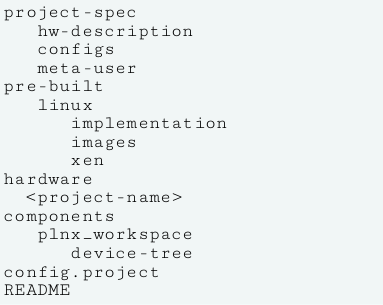
\includegraphics[width=0.7\textwidth]{./images/petalinux-projektstruktur.jpg}
	\end{center}
	\vspace{-5pt}
	\caption[petalinux Projektstruktur]{typische petalinux projektstruktur [\cite{petailinuxtool}]} % Eckige Klammer (optional): Caption-Text in Abbildungsverzeichnis
	\label{fig:petalinux:projektstruktur}
	\vspace{-5pt}
\end{figure}
In Abbildung ~\ref{fig:petalinux:projektstruktur} ist eine typische Petalinux Projektstruktur dargestellt. 

\begin{itemize}
	\item \textbf{project-spec}: In diesem Verzeichnis werden alle Änderungen an dem Projekt durchgeführt. Hier können z. B. neue Projekt Layers erstellen, den Gerätebaum(Device-tree) geändert oder sogar Rezepte für Software, die vom Kernel kompiliert werden soll, erstellt werden. 
	\item \textbf{pre-built}: Dieses Verzeichnis beinhaltet alle Board-spezifischen Design- und Konfigurationsdateien, vorgefertigte und getestete Hardware und Software-Images, die Sie auf Ihr Board direkt heruntergeladen werden können. Der Ordner ist jedoch nur sichtbar, wenn man das Projekt auf der Basis des für das Board spezifischen Board Support Package (BSP) erstellt haben. 
\end{itemize}
